\apendice{Planificación}

\section{Introducción}
En el desarrollo de este proyecto, utilizaremos la metodología SCRUM, con un desarrollo incremental con una duración de 2 semanas por Sprint. 
La organización en GitHub se realizará del siguiente modo: 
\begin{itemize}
\item Creación de un nuevo Milestone con una duración de 2 semanas el día de la reunión. 
\item Creación de los issues básicos necesarios para dicho Milestone. 
\item Desarrollo de los issues y la creación de los nuevos issues necesarios. 
\item Utilización de la herramienta Zenhub para el seguimiento de las tareas. 
\item Cierre de las issues una vez finalizadas para observar el avance de las tareas de forma real frente al progreso ideal. 
\end{itemize}

\section{Planificación temporal}
La evolución bisemanal de las tareas se ha realizado de la siguiente manera: 
\subsection{\textbf{Sprint 1}  (15/01/2018-29/01/2018) }
El primer Sprint, orientado hacia la explicación del desarrollo del proyecto. Se decidirán las herramientas básicas de la gestión de tareas, documentación de memoria y anexos y las referencias bibliográficas. 
Por ello: 
\begin{itemize}
\item Se ha documentado y probado la utilización de \LaTeX como editor de texto.
\item Se han documentado y probado los gestores de versiones de metodología ágil. 
\item 

\end{itemize}
\subsection{\textbf{Sprint 2}  (29/01/2018-12/02/2018) }
El segundo Sprint, orientado hacia las técnicas utilizadas en \LaTeX así como las diferentes asígnaturas existentes en el Grado de Ingeniería Informática. Durante la reunión, se decidirá el tipo de cuestionario a realizar, y cómo orientarlo hacia la recogida de datos.  
Por ello: 
\begin{itemize}
\item Se ha comenzado el desarrollo de la Memoria en \LaTeX  y la documentación del mismo. 
\item Se han documentado las diferentes asignaturas existentes. 
\end{itemize}
\textbf{Problemáticas encontradas}\\En el segundo Sprint,hemos tenido el mismo problema que en el Sprint 1, teniendo en cuenta los "Estimate" como la dificultad, sin tener en cuenta que algunas tareas, a pesar de ser sencillas, tienen una mayor duración de tiempo. \\Además, nos hemos encontrado con menor tiempo, por lo que hemos tenido que transpasar un Issue al Sprint 3. \\Finalmente, hubo una confusión en el "Due Date", ya que habíamos considerado como el tiempo de comienzo en lugar del tiempo de fin. Dicho error fue corregido en el Sprint 3.

\begin{figure}[h]
\centering
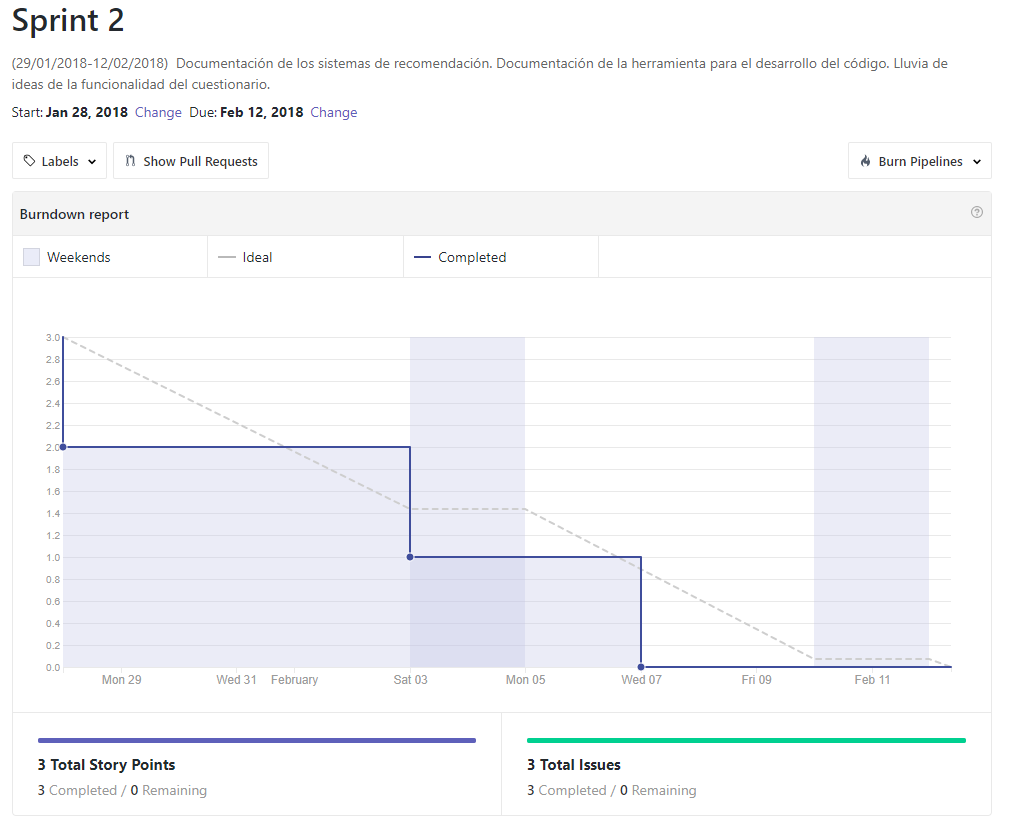
\includegraphics[width=0.99\textwidth]{Sprint_2}
\caption{Burndown del segundo Sprint}
\label{fig:A.2.1}
\end{figure}


\subsection{\textbf{Sprint 3}  (13/02/2018-27/02/2018) }
El tercer Sprint, se ha orientado hacia la terminación del Sprint 2, ya que, por falta de tiempo, no se terminaron las issues. 
Por ello: 
\begin{itemize}
\item Se ha creado el formulario y distribuido entre los diferentes ex-alumnos del Grado de Ingeniería Informática en Burgos. 
\item Se ha documentado la metodología de integración de las funcionalidades del cuestionario y cómo almacenar los datos. 
\item Se ha realizado una documentación de los diferentes sistemas de Recomendación existentes.  
\end{itemize}
\textbf{Problemáticas encontradas}\\En el tercer Sprint,hemos tenido el mismo problema que en el Sprint 1 y 2, teniendo en cuenta los "Estimate" como la dificultad, sin tener en cuenta la duración del mismo.\\Por otro lado, al igual que en el Sprint 1 y el Sprint 2, no cerramos correctamente el Milestone, de forma que fue cerrado una vez comenzado el Sprint 4, a pesar de que las Issues se encontraban ya cerradas.

\begin{figure}[h]
\centering
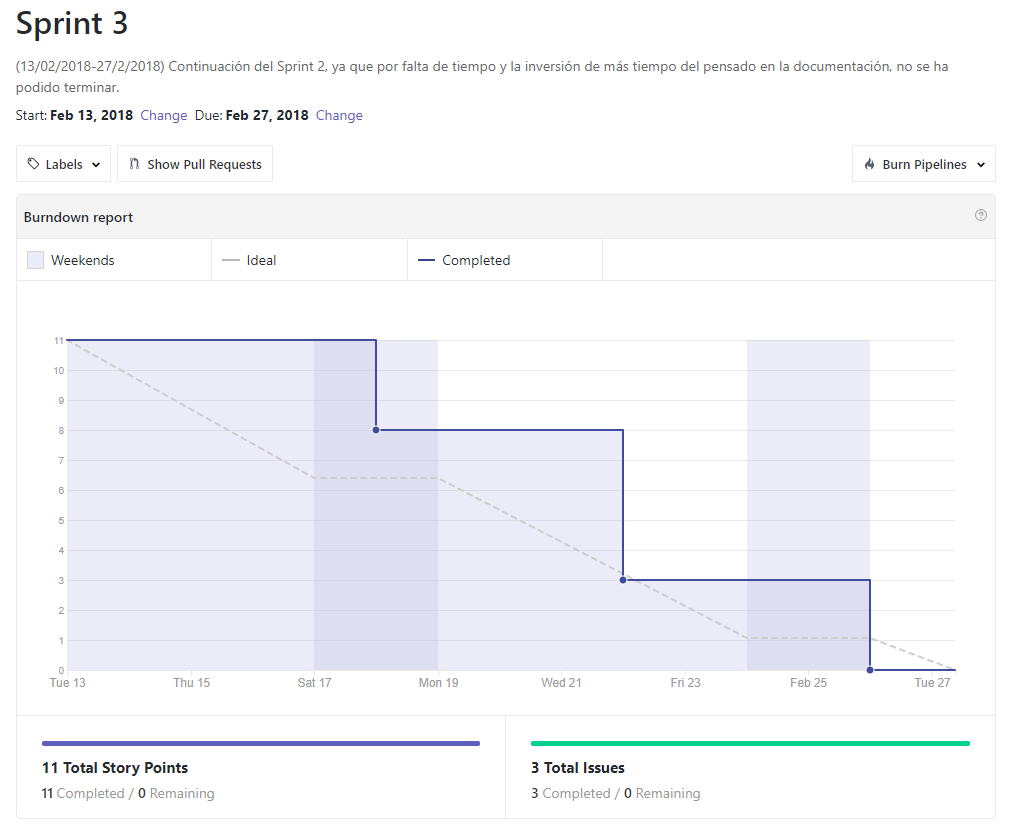
\includegraphics[width=0.99\textwidth]{Sprint_3}
\caption{Burndown del tercer Sprint}
\label{fig:A.2.1}
\end{figure}


